\documentclass[a4paper]{article}

\usepackage[utf8]{inputenc}

\usepackage{url}
\usepackage{hyperref}

\usepackage{caption}

\usepackage{listings}

\usepackage{color}

% *** GRAPHICS RELATED PACKAGES ***
%\usepackage[pdftex]{graphicx}
\usepackage{graphicx}
%\usepackage[dvips]{graphicx}
% to place figures on a fixed position
\usepackage{float}

\usepackage[margin=1in]{geometry}

\title{P2P – syllabus}
\author{}
\date{}


\begin{document}

\maketitle

\tableofcontents

\section{Introduction}

Compared to traditional client-server operation peer-to-peer solutions (P2P) offer a more direct and dynamic
solution. They provide searching services in a global network and allow direct, point to point data transfers
bypassing the administrative and performance bottlenecks of servers.
The well-know and most used P2P applications -- like file exchange, VoIP and on-line gaming -- affects many users and
generate the significant portion of today's Internet traffic. Covering all aspects of P2P network during this lab would
be impossible therefore only some key parts will be demonstrated. Since file transfer is currently to most utilized
application we are going to cover that during this lab.

\section{P2P file exchange}

The first system specifically designed for file exchange called \emph{Napster} was released in 1999. The file exchange
networks were growing rapidly after that, several architectures had been developed and had been categorized  into 3
main categories. This chapter gives an overview on each and then discusses BitTorrent in detail which is going to be
the main focus during this lab.

\subsubsection{Client-server systems}

The architecture of Napster is considerably simple. The basis of it is one central server and each user is connected to
this server with its client program. Downloading is controlled by the central server however the data transfer is
between the two requesting and the offering clients directly without going through the server. This property makes it
eligible Napster to be categorized as a P2P network due to utilizing the storage capacity and network access bandwidth
of all of its clients. An obvious shortcoming of Napster's architecture is the reference to the central server park --
shutdown of that would bring down the whole network. This had happened several times in the past due to ongoing legal
procedures between RIAA (American copyright protection entity) and Napster because of the contents that were available
on the network.

The focus transitioned on changing the principal design of the architecture and was looking for a solution that doesn't
rely on central entities i.e. it's fully distributed. Others were just trying to address security related problems. The
resulting architecture had the clients connect to a server but the server itself did not store an information about the
clients and many smaller servers were in operation instead of just one central entity. The most notable implementation
of this architecture is DirectConnect.

\subsubsection{Distributed systems}

After the fall of Napster it had been realized that the main vulnerability of these systems is the presence of the
central server. Later on as a result of repeated strikes against DirectConnect based networks most of the file exchange
users started looking for a system which operates in a fully distributed way i.e. it doesn't have any central entity.
The distributed architecture had its own cons compared to the client-server based approach. In distributed systems the
number of network hops could be arbitrarily large resulting in greater network traffic in the network itself and in
increased execution time of downloads, queries, etc. Another theoretical problem is that connecting to a distributed
network is not trivial -- due the missing central server -- the client who wants to connect has to obtain the network
address of some already connected client. Furthermore network administration had become virtually unmanageable.

Around the year 2000 several networks had been operated based on the principles described above. Almost every
programmer was developing P2P file exchange software in his free time. A variety of different but short-lived solutions
had been introduced in this era. However some of the systems have survived and gain popularity for example Gnutella
which is still one of the most popular network in some countries.

Gnutella network is truly peer-to-peer which means that its only contains clients communicating with each other; it
doesn't utilize any central or globally reachable component. As mentioned before there is a problem arising from new
client connections: it's necessary to know at least one already connected client. Initially there was no well
established methodology for that resulting in spreading the word about some clients that were already connected between
people to be able to connect to the network. There had been some search algorithms introduced to overcome this however
these did not operate effectively in global scale.

After a client got hold of a Gnutella member it could initiate a connection to it with a greeting message. The peer
receiving this message replies and indicates its availability. Furthermore it forwards the message to all of its known
peers - naturally these messages utilized a Time-To-Live (TTL) mechanism. This process repeats until the TTL reaches 0.
During the message's lifetime it gets process by a lot of network members -- technically all peers in 6 hops distance
from the edge peer. Afterwards the connecting peer initiates a connection to all reachable peers as a result then it is
tightly coupled to the network.

Gnutella provides almost complete security against legal concerns because the complete network is technically
non-discoverable. This non-discoverable property is one of the greatest drawbacks of it because due to the client's
relatively small horizon it it impossible to know many peers are using the network without being able to monitor the
whole Internet. Still there are only approximations about the total number of users which says it's around the
magnitude of 1000 connection per 1 peer.

The search messages are processed similarly to the connection initiation messages. The client floods the search message
to all of its connected peers. Those process the query and if any has a positive match it sends back a reply. The
message is then flooded onwards -- TTL mechanism still applies. In this way the search request	traverses all the way
through the client's horizon and the originating peer receives all the positive matches. The reply messages may contain
new peers that can be used for establishing new connections if the originating peer would like to broaden its horizon.

\subsubsection{Hierarchical systems}

The hierarchical systems combine the advantages of the previously described client-server and pure P2P networks.
It doesn't have central entities with global availability however not all peers are equal: some of the entities has
special responsibilities.
This type of network can be imagined as the special purpose entities -- a.k.a. super-clients -- are connected to each
other in a P2P fashion while regular clients are connected to these super-clients in a client-server fashion.
Kazaa (FastTrack) operates based on this principle.

Fastrack is basically based on later versions of Gnutella where only the \emph{Ultrapeers} are eligible to be connected
to the Gnutella network itself while the leaf clients can only connect to Ultrapeers. The Ultrapeers responsibility
beside processing their own search operations is to serve the connected regular clients and take over their traditional
P2P tasks. In the Kazaa network the Ultrapeers are called \emph{Superpeers}.

When the user starts the client program that uses a proprietary algorithm to decide the role in which it will operate.
If it is going to be a Supernode it is trying to establish connections with other Supernodes. Due to the encrypted
communication it is unknown how Supernodes find each other but it's known that the client software contains a
hard-coded list of Supernodes that gets updated with each release. The Supernode under connection tries to connect to
Supernodes chosen from this list until it successfully connects to one of them. After successful connection the other
Supernodes will send the current list of Supernodes in the network so the newly connected Supernode can update its
database. It is unknown that how the list of Supernodes is created but it's likely that it is similar to the process
used by Gnutella. The protocol used between Supernodes are not known in details due the encrypted nature of the
communication but measurements showed that a Supernode connects to 25 other Supernodes on average.

FastTrack architecture is a fine fusion between the client-server and the pure P2P networks. The Supernodes backbone
that replaces the central server entity provides a scalability and high-availability. Flooding only takes part between
Supernodes as a consequence as more ordinal peers connect to the network the network traffic is not growing
proportionally -- it only increases between the high bandwidth Supernodes. This architecture resembles the architecture
of Skype -- not accidentally as the same developer team was responsible for developing both systems.

\section{BitTorrent}

The original purpose of BitTorrent released in 2001 was to decrease the load on servers. The problem to solve is that
given a server there are too many clients trying to download the same file. The sever slows as more and more clients
connects to it and in worst case it could crash. The key idea behind BitTorrent is that the clients could download
fragments of data from other clients as soon as the have it. The files are fragmented into smaller chunks that are
eligible to be download in any order, and not only from the server but from other clients that has the corresponding
fragments as well. As more and more clients download a fragment/piece from each other it will have greater availability
reducing the server load proportionally. The implementation uses two central functionality: the \emph{Seeder} is a
server that originally provided full access to the original file; the \emph{Tracker} is also a server that track the
downloading process so it can provide information on fragment availability -- which fragment can be downloaded from
which clients -- for the newly connected clients.

In terms of network size this concept is a refinement of the transition between Napster and DirectConnect. While
Napster aimed for a globally uniform network DirectConnect focused on creating smaller, topic based networks. These
kind of smaller networks received connections from clients who were interested in the content of the specific topic
provided by the network as a result reducing the number of ``unnecessary" files shared on a single network. BitTorrent
continues along this basic concept to an extreme where micro networks are established for sharing a single file.
Naturally one client can be a part of several of these networks still it only has to be a member of those in which it
has interest in. This hypothesis is backed by measurements -- in a file sharing system the 90\% of the traffic is
generated by the 5-10\% of the files shared.

Due to this property the system offers extremely fast download speeds where most of the time the bottleneck is the
downlink bandwidth of the client's access network. Despite its differences compared to the other file sharing solutions
the potential of BitTorrent has been realized quickly. There were minor modifications in the implementation but thanks
to the open source nature of the project new releases were published repeatedly that offered better and better file
sharing capabilities from release to release. To be specific the main function of it was file downloading since it
didn't have any other features.

For practical reasons due to file sharing the following modifications had been done: there are special purpose web
sites from where the users can download torrent files. These sites can vary but the same torrent file can be found on
multiple sites. Based on the torrent files the client can find the appropriate Tracker and Seeder servers.

Another speciality is the Seeder server doesn't have a distinguished role. In this variant a client that has finished
downloading -- i.e. it has all the fragments of a file -- it becomes a Seeder itself. As time progresses the number of
Seeders will increase in the network further increasing the download speed. Despite the Seeder server the terminology
calls Seeders those clients as well which are sharing the complete files for the other clients.

In order to connect to the network the user downloads the torrent file and the BitTorrent client can use that to locate
the file's Tracker and Seeder servers. Using the Tracker the client can find other clients that has only downloaded
fragments of the current file so they are also eligible to download from. In newer versions the torrent file can refer
to multiple Tracker and Seeder servers as a result providing higher availability in case of a server outage.

The content sharing is done slightly differently compared to other P2P file sharing networks. BitTorrent had been
developed for sharing specific files and content not for sharing more and more files as a consequence it does not
support sharing full folders.

To be able to share first one has to select one (or more) Tracker server. After the Tracker has been selected a torrent
file has to be created that refers to the creator host as Seeder and to the chosen Tracker server as Tracker.
Furthermore the candidate file to be shared has to be fragmented into pieces with corresponding hash information
calculated and written into the torrent file. Finally the torrent file has to be published for example on some of the
well-known sites in order to be found by those whom are interested in the content. Some of the web-sites provide
searching services if some of the meta-data are also given.

As soon as the clients obtain fragments of the file they are sharing it wit the other by notifying the Tracker server
that they also have that particular segment. After the full file has been downloaded the client becomes a Seeder and it
can appear as a potential seeder in the torrent file.

Nonetheless the client programs are open source most of them prevent ``free-riding" i.e. the download bandwidth should
be proportional to the upload bandwidth in order to restrict leeching on the other clients.

Since in case of BitTorrent there are so-called micro-network that are specifically established to broadcast a given
file there are no means to execute queries for specific files. Search operations usually provided by those web-sites
that are specialized in storing torrent files. On these servers one can save auxiliary meta-data for any torrent file
so it can be searched through the web UI. In practice a search results in a torrent file that leads the client to the
corresponding file-sharing micro-network.

Furthermore the client can connect to a Tracker server using the info obtained from the torrent file. The Tracker then
directs the client to those other clients and Seeders from where fragments of the given file can be downloaded. After a
piece has been downloaded the Tracker records it as a result subsequent clients can download the same fragment from the
previous client.

Actually the fragments of a file are further divided into smaller pieces so even in case of short availability shared
full downloads can be successful. If a client successfully obtain a sub-fragment of a fragment the software will give
precedence to download other sub-fragments from the same fragment. Given this algorithm it's more likely to obtain full
segments that are eligible to be downloaded by others. The integrity of a fragment is verified by checking the
calculated has value of the downloaded fragment with the one present in the torrent file. Another optimization is that
the Tracker counts that which fragment has the lowest availability in the network and it directs a newly connected
client to download those fragments. This results in off-loading the server and on the other hand it also provides high
availability of the file in the network so in case of the Seeder is lost the rare segments could be downloaded as well.
Nevertheless clients benefit from downloading fragments with low availability since as soon as it obtains such a piece
it will be selected as an uploader with higher probability. This ensures more downloader and provides greater global
download bandwidth as well as greater download bandwidth for itself. To summarize the file downloading works like the
client connect to as many clients -- that have full fragments available -- as possible and as soon as the downloading
client obtains a full fragment it shares it and provides availability for these fragments.

The time that takes to download files varies greatly it's almost unpredictable. Slow start of download characterizes
the system that is followed by exponential speed-up. In the beginning only the Seeder has the file as a result all
clients will download from that. As time passes more and more peers will have fragments available thus off-loading the
server gradually and providing more and more upload bandwidth for the given file.

Torrent file use \emph{bencode} for encoding data. This is a string based encoding that can be decoded easily. This
encoding supports two primitive types and one complex type. The primitive types can be used for storing strings and
integers respectively and the complex types can be used for building lists and dictionaries. Recursive composition of
complex types is supported -- e.g. a list can contain another list as an element.

The integers are represented by writing the number to be encoded between  a leading ``i" and a trailing ``e" -- e.g
`13' is encoded as `i13e'.

Strings are encoded in way that the length of the string is written before a colon that is followed by the actual
string. For example the string ``apple" in encoded format is `5:apple'. Important to notice that there is no terminator
that follows the string, the length of the string can be determined from the leading length indicator.

List can contain arbitrarily many entries that are encoded between a leading ``l" and a trailing ``e" character. For
example ``l5:applei13ee" encodes a list of two where the first element is the string ``apple" that is followed by the
number `13'.

Dictionaries -- similarly to lists -- are encoded between leading ``d" and a trailing ``e" character however the number
of elements must be an integral multiple of 2 where the fist element of a pair is going to be the key and the second
will be the value. For example the ``d5:applei13e4:pear4:null" encodes a dictionary that assigns the number `13' to the
string key ``apple" and has value string ``null" assigned to the key ``pear".

\section{Topology-aware BitTorrent clients}

Even though P2P applications had grown rapidly currently their importance is declining though they still have an
important role in today's Internet traffic: approximations are that P2P applications generate almost 70\% percent of
the total traffic of the Internet at some time point. The problem is that this overlay concept ignored the network
topology. BitTorrent  -- which is the most popular client nowadays -- greatly increases the cost that is spent on
inter-provider links by the Internet Service Providers (ISP). This forces the ISPs to restrict and/or shape P2P traffic
in their network which results in dissatisfied users.

Topology-aware P2P applications try to address this problem.

Ono is a Vaze BitTorrent client plug-in that instead of randomly selecting a peer -- from topology perspective -- it
aims to find peers that are considered to be near. Those neighbouring peers are expected to have smaller latency and
greater bandwidth and also reducing inter-ISP and backbone traffic. The Ono plug-in measures peer proximity using
measurement results from content delivery networks (CDN) e.g. Akami.

The TopBT client performs active discovery of neighbouring peers and it takes also into account transmission bandwidth
in order to provide high download speeds via short network hops as result reducing the total Internet traffic. TopBT
uses \emph{ping} and \emph{traceroute} utilities to measure the proximity of other peers. Compared to Ono there is no
need for getting measurement data from ISPs or CDN providers and doesn't require other clients to run TopBT as well.

\section{P2P network using Mininet, OpenFlow switches and POX controller}

The introduction to Mininet, OpenFlow and POX controller can be read in the OpenFlow \& Mininet syllabus. On
Figure~\ref{fig:Lab-topo} the network topology used in this P2P lab is shown.

\begin{figure}[H]
    \centering
    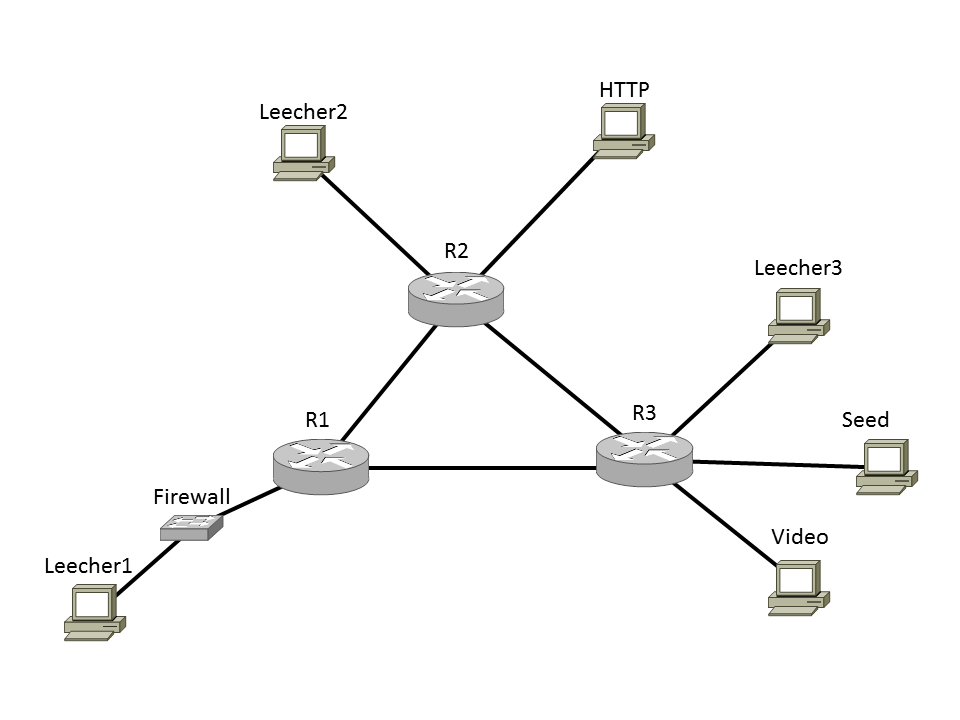
\includegraphics[width=0.9\textwidth]{figures/halozat.png}
    \caption{Network architecture used in lab exercises}
    \label{fig:Lab-topo}
\end{figure}

There are 4 OpenFlow switches running in the network of those 3 (R1,R2,R3) are implementing an IP router with static
routes. Important to note that these OpenFlow switches are not capable to respond to ARP requests so those have to be
handled from an appropriate controller application or alternatively use static MAC addresses -- the latter is used in
this lab exercise. In this network setting the hosts can reach their gateways on all-zero MAC address (by the way that
is an invalid MAC address). The host MAC addresses are composed from the scheme
``00:00:\textless~ROUTER-ID~\textgreater:00:00:~\textless~ROUTER-LINK-ID~\textgreater. Given these as example the fist
host (leecher 2) connected to R2 router has
MAC address ``00:00:02:00:00:01".

The R2 router has the following flow entries programmed:

\begin{lstlisting}[language=bash,frame=single,breaklines,caption={R2 router flow entry configuration},label=lst:R2-flow-config]
ovs-ofctl add-flow r2 'ip,nw_dst=89.97.0.0/16,action=mod_dl_src:00:00:00:00:00:00,output:4'
ovs-ofctl add-flow r2 'ip,nw_dst=201.42.54.65/28,action=mod_dl_src:00:00:00:00:00:00,output:5'
ovs-ofctl add-flow r2 'ip,nw_dst=23.53.32.53/32,action=mod_dl_dst:00:00:02:00:00:01,output:1'
ovs-ofctl add-flow r2 'ip,nw_dst=23.99.30.4/32,action=mod_dl_dst:00:00:02:00:00:02,output:2'
ovs-ofctl add-flow r2 'ip,nw_dst=23.0.3.78/32,action=mod_dl_dst:00:00:02:00:00:03,output:3'
ovs-ofctl add-flow r2 'arp,action=output:1,2,3' 
\end{lstlisting}

The first two rules covers for the two adjacent router's IP range. It can be seen that those networks have a /16 and
/28 subnet mask. If an IP packet is destined to a host in these subnets then a source MAC address change will occur and
the packet is sent out on the appropriate output port -- for proper operation the destination MAC address has to be
changed as well but in this case it can be omitted since the other end is also an OpenFlow switch programmed using this
principle.
For the hosts there is only a full match when all 32 bits of the IP destination address matches the flow entry's
destination IP address. If there is a match for the hosts the destination MAC is swapped to the host's MAC address and
the packet is sent out towards the host. The last entry serves the purpose of forming a broadcast domain from ports
1,2,3 since some of the ARP packets are destined to the broadcast MAC address and has to be flooded. However the
flooded packets must only be flooded in the same broadcast domain as on they arrived. If the flooded packets were
transmitted on all ports  -- towards the routers as well -- it would paralyze the Mininet network emulation by the
resulting in broadcast storm.

The 4th switch operating as a Firewall doesn't have static OpenFlow entries it is solely controlled by the controller.
The lab exercise is to program filtering logic into the Firewall so that it properly filters or shapes the torrent
traffic. The firewall has two ports and it implements a repeater by default that is forwarding the packets arriving on
it's input port as-is on the output port that is implemented in the POX controller's \emph{handlePacketIn} method. The
desired operation has to be also implemented in this method. The parsing of the incoming packets are done by this call
\begin{lstlisting}[language=python,frame=single,breaklines]
packet = event.parsed  
\end{lstlisting}

From there the `packet' object can be easily queried for well-known OpenFlow parameters. Like for example the input
port id is in the filed `packet.port' and finding a specific TCP port from the packet could look like this:

\begin{lstlisting}[language=python,frame=single,breaklines]
tcpp = event.parsed.find( 'tcp' )

if not tcpp: return # Not TCP

if tcpp.srcport in block_ports or tcpp.dstport in block_ports:

# Halt the event, stopping l2_learning from seeing it

# (and installing a table entry for it)

core.getLogger( "blocker" ).debug( "Blocked TCP %s <-> %s" ,tcpp.srcport, tcpp.dstport)

event.halt = True
\end{lstlisting}

Since OpenFlow does not parse the packet above L4 parsing a BitTorrent packet header requires more work by analyzing
the L4 payload using the `payload' property of the object.

\appendix

\section{Entry quiz sample questions}
\begin{itemize}
    \item When was the appearance of the P2P paradigm dated? What were the motivators behind it? What are the main
          categories of P2P applications?
    \item What is the most popular P2P file sharing technology currently? What are the components of the system? What is
          the principle of its operation?
    \item What is the problem of the ISPs with P2P applications (beside copyright issues)? What solutions had appeared
          to overcome those problems?
    \item How does the ISPs fight against the P2P traffic and what are the reactions of the P2P clients?
\end{itemize}

\section{Input files for the lab exercise}
\begin{itemize}

    \item \href{https://qosip.tmit.bme.hu/foswiki/pub/Meres/P2PAlkalmazasokMeresiSegedlet/p2pMeresTopo.py.txt}
          {p2pMeresTopo.py.txt}: Mininet topology for the P2P measurements, run by executing: `sudo python
          p2pMeresTopo.py'

    \item \href{https://qosip.tmit.bme.hu/foswiki/pub/Meres/P2PAlkalmazasokMeresiSegedlet/p2pMeresTopo.py.txt}
          {p2p.py.txt}: POX controller application to be copied into pox/ext directory, run by executing: `./pox.py p2p'

\end{itemize}

\section{Lab exercises}

\subsection{Setting-up the measurement environment}
\begin{enumerate}
    \item Select `P2P' option from the boot menu
    \item VirtualBox settings
          \begin{enumerate}
              \item Under Settings/Network change `Adapter 1' to `NAT' (NOT NAT Network!)
              \item Under VBox Settings/System/Motherboard tick `Enable I/O APIC'
              \item Start the image
          \end{enumerate}
    \item Ubuntu settings
          \begin{enumerate}
              \item Start a terminal and disable Network Manager with executing `sudo service network-manager stop'
                    command. Then execute `sudo dhclient eth0' to restore the NAT IP address
              \item Start the controller using the command `pox/pox.py p2p' command (pox is under /home/p2p/pox/).
                    The INFO logs can be filtered by passing `log.level --WARNING' startup argument, but in this case the own log messages
                    has to be logged at least on log level warning
              \item Start Mininet with command `sudo python p2pMeresTopo.py' (the mininet topology script can be
                    found under directory /home/p2p/)
          \end{enumerate}
    \item Mininet setup
          \begin{enumerate}
              \item Verify connections using command 'pingall' from the Mininet shell
              \item From the mininet shell start xterm windows on the selected hosts (e.g `xterm Leecher1 Leecher2
                    Leecher3 Seed')
              \item Set the home directory on each host (Leecher1-3,Seed) by executing the command `export
                    HOME=/home/p2p/\textless~HOST NAME~\textgreater' from the corresponding xterm window
          \end{enumerate}
\end{enumerate}

\subsection{Measuring the effects of access network bandwidth}
\begin{enumerate}
    \item Generate a big file and create a torrent file from it
          \begin{enumerate}
              \item An 500MB file can be created quickly by executing `dd if=/dev/zero
                    of=/home/p2p/Seed/big\_file.txt count=1024 bs=524288'
              \item It is recommended to use qbitorrent application: it has a built-in tracker function that has to
                    be enabled under settings/special (listens on port 9000 by default)
              \item when creating the torrent file specify the Tracker as ``http://\textless~IP
                    address~\textgreater:\textless~Tracker port~\textgreater~/announce"
              \item it is advised to immediately seed the file on host \emph{Seed}
          \end{enumerate}
    \item  Download torrent file to hosts Leecher1-3 and start downloading
          \begin{enumerate}
              \item It is recommended to use `uTorrent' client
              \item The path under which the file is downloaded is advised to be set under the recently exported
                    \$HOME directory (/home/p2p/Leecher1). The simplest is to start uTorrent from the \$HOME directory so it will download
                    files there by default.
              \item start uTorrent using command `utserver -settingspath /opt/utorrent-server-alpha-v3\_3/ \&' and
                    the GUI can be accessed through \url{http://localhost:8080/gui} . The user name is `admin' and there is no password.
              \item The GUI has to be started on the corresponding hosts to have it running in the appropriate
                    namespace. For example accessing uTorrent running on Leecher1 is possible from a Firefox started on host Leecher1.
                    Close Firefox between setting up downloads as it will continue to use the existing sessions.
          \end{enumerate}
    \item Start web and video server on hosts HTTP and Video
          \begin{enumerate}
              \item a simple web server can be started from python's built-in SimpleHTTPServer  with `python -m
                    SimpleHTTPServer'
              \item The video streaming has to be started on host Video using the script from
                    listing~\ref{lst:video-stream} that streams the screen over HTTP on port 8080
          \end{enumerate}
    \item Measuring real-life like traffic on host Leecher1. For this \textbf{simultaneously} run P2P download, web
          requests and video streaming
          \begin{enumerate}
              \item To start web requests use the script from listing~\ref{lst:web-requests} . It's advised to create
                    a file called `small\_file.txt' on the web server before starting the script
              \item start the video client: Connect to the VLC network stream using VLC media player on
                    ``http://\textless~Server IP address\textgreater:8080"
              \item in case if the P2P has finished in the meantime then delete the file and restart the download
          \end{enumerate}
    \item Use Wireshark on host Leecher1 to analyze the network traffic
    \item Change the access network bandwidth from the default 10Mbps to 5Mbps and subsequently to 1Mbps while
          repeating the capture and analysis above. For this use `wondershaper' shown in listing~\ref{lst:wondershaper}
          (Note:wondershaper has to be installed!)

          \begin{lstlisting}[language=bash,frame=single,breaklines,caption={VLC streaming server command},label=lst:video-stream]
vlc-wrapper -Idummy screen:// :screen-fps=30 :screen-caching=100 --sout '#transcode{vcodec=mp4v,vb=4096,acodec=mpga,ab=256,scale=1,width=1280,height=800}:http{port=8080,mux=ts}' 
\end{lstlisting}

          \begin{lstlisting}[language=bash,frame=single,breaklines,caption={Automatic HTTP download script},label=lst:web-requests]
#!/bin/sh

while true; do

wget http://23.0.3.78:8000/small_file.txt -o /dev/null

sleep 1

done 
\end{lstlisting}

          \begin{lstlisting}[language=bash,frame=single,breaklines,caption={Adjusting link capacity},label=lst:wondershaper]
wondershaper Leecher1-eth0 1024 1024 
\end{lstlisting}

\end{enumerate}

\subsection{Throttling P2P traffic from ISP side}
\begin{enumerate}
    \item Implement blocking of P2P traffic on Firewall device using the OpenFlow POX controller attached to it
          (\$HOME/pox/ext/p2p.py) -- hint: traffic ports, and header bits
    \item Document the test results of the implemented traffic throttling application
    \item Rewrite the throttling application in a way that it can be used for traffic shaping: Restrain P2P
          download bandwidth to 1Mbps on average
    \item Document the test results of the shaping application
\end{enumerate}

\subsection{ISP response for advanced P2P file sharing settings}

\begin{enumerate}
    \item Use random port selection in the torrent client (and restart it multiple times), use encryption
    \item Evaluate and improve the previously written throttling and shaping applications
\end{enumerate}

\end{document}